\documentclass[11pt]{article}
\usepackage[review]{acl}
\usepackage{times}
\usepackage{latexsym}
\usepackage[T1]{fontenc}
\usepackage[utf8]{inputenc}
\usepackage{microtype}
\usepackage{inconsolata}
\usepackage{graphicx}
\usepackage{booktabs}
\usepackage{amsmath}
\usepackage{xspace}
% generated by paper_tables.py
\newcommand{\R}[1]{\ifcsname r@#1\endcsname\csname r@#1\endcsname\else\textbf{??}\fi}
\expandafter\def\csname r@auth.dir.hi\endcsname{85}
\expandafter\def\csname r@auth.dir.lo\endcsname{66}
\expandafter\def\csname r@auth.dir.med\endcsname{80}
\expandafter\def\csname r@auth.ver.hi\endcsname{86}
\expandafter\def\csname r@auth.ver.lo\endcsname{75}
\expandafter\def\csname r@big.bbeh.auth.dir\endcsname{100}
\expandafter\def\csname r@big.bbeh.auth.ver\endcsname{100}
\expandafter\def\csname r@big.bbeh.gap\endcsname{+4.6}
\expandafter\def\csname r@big.bbeh.gap0\endcsname{+6.0}
\expandafter\def\csname r@big.bbeh.knows\endcsname{63.2}
\expandafter\def\csname r@big.bbeh.pool.cot.rank.ci\endcsname{$-$0.7 [$-$5.4, +4.2]}
\expandafter\def\csname r@big.bbeh.pool.cot_sum.rank.ci\endcsname{+3.9 [$-$1.1, +8.6]}
\expandafter\def\csname r@big.bbeh.pool.direct.rank.ci\endcsname{+6.0 [+1.2, +11.0]}
\expandafter\def\csname r@big.bbeh.pool.sum.rank.ci\endcsname{+4.5 [+1.6, +7.4]}
\expandafter\def\csname r@big.bbeh.pool.x11.rank.ci\endcsname{+1.4 [$-$1.2, +4.0]}
\expandafter\def\csname r@big.bbeh.pool.x4.rank.ci\endcsname{+1.0 [$-$0.4, +2.5]}
\expandafter\def\csname r@big.bbeh.says\endcsname{58.6}
\expandafter\def\csname r@big.bbeh.sm.qwen.cot.rank.abs\endcsname{58.0}
\expandafter\def\csname r@big.bbeh.sm.qwen.cot.rank.ci\endcsname{+2.8 [$-$0.1, +5.4]}
\expandafter\def\csname r@big.bbeh.sm.qwen.cot_sum.rank.abs\endcsname{56.6}
\expandafter\def\csname r@big.bbeh.sm.qwen.cot_sum.rank.ci\endcsname{+1.4 [$-$1.6, +4.4]}
\expandafter\def\csname r@big.bbeh.sm.qwen.direct.rank.abs\endcsname{56.1}
\expandafter\def\csname r@big.bbeh.sm.qwen.direct.rank.ci\endcsname{+0.9 [$-$2.4, +4.2]}
\expandafter\def\csname r@big.bbeh.sm.qwen.nq\endcsname{311}
\expandafter\def\csname r@big.bbeh.sm.qwen.sum.rank.abs\endcsname{57.8}
\expandafter\def\csname r@big.bbeh.sm.qwen.sum.rank.ci\endcsname{+2.6 [+0.4, +4.9]}
\expandafter\def\csname r@big.bbeh.sm.qwen.verdict.rank\endcsname{55.2}
\expandafter\def\csname r@big.bbeh.sm.qwen.x11.rank.abs\endcsname{54.7}
\expandafter\def\csname r@big.bbeh.sm.qwen.x11.rank.ci\endcsname{$-$0.5 [$-$2.6, +1.6]}
\expandafter\def\csname r@big.bbeh.sm.qwen.x4.rank.abs\endcsname{56.1}
\expandafter\def\csname r@big.bbeh.sm.qwen.x4.rank.ci\endcsname{+0.9 [+0.0, +1.9]}
\expandafter\def\csname r@big.bbeh.solved\endcsname{15}
\expandafter\def\csname r@big.math.auth.dir\endcsname{72}
\expandafter\def\csname r@big.math.auth.ver\endcsname{76}
\expandafter\def\csname r@big.math.gap\endcsname{+4.5}
\expandafter\def\csname r@big.math.gap0\endcsname{+4.4}
\expandafter\def\csname r@big.math.knows\endcsname{66.3}
\expandafter\def\csname r@big.math.pool.cot.rank.ci\endcsname{+0.7 [$-$1.5, +2.9]}
\expandafter\def\csname r@big.math.pool.cot_sum.rank.ci\endcsname{+3.8 [+1.9, +5.8]}
\expandafter\def\csname r@big.math.pool.direct.rank.ci\endcsname{+4.4 [+2.3, +6.5]}
\expandafter\def\csname r@big.math.pool.sum.rank.ci\endcsname{+2.6 [+1.2, +3.9]}
\expandafter\def\csname r@big.math.pool.x11.rank.ci\endcsname{+0.5 [$-$1.2, +2.1]}
\expandafter\def\csname r@big.math.pool.x4.rank.ci\endcsname{+1.7 [+0.5, +2.9]}
\expandafter\def\csname r@big.math.says\endcsname{61.9}
\expandafter\def\csname r@big.math.sm.olmo.cot.rank.abs\endcsname{62.8}
\expandafter\def\csname r@big.math.sm.olmo.cot.rank.ci\endcsname{+0.2 [$-$5.0, +5.8]}
\expandafter\def\csname r@big.math.sm.olmo.cot_sum.rank.abs\endcsname{63.1}
\expandafter\def\csname r@big.math.sm.olmo.cot_sum.rank.ci\endcsname{+0.5 [$-$3.3, +4.1]}
\expandafter\def\csname r@big.math.sm.olmo.direct.rank.abs\endcsname{64.4}
\expandafter\def\csname r@big.math.sm.olmo.direct.rank.ci\endcsname{+1.8 [$-$1.7, +4.9]}
\expandafter\def\csname r@big.math.sm.olmo.nq\endcsname{89}
\expandafter\def\csname r@big.math.sm.olmo.sum.rank.abs\endcsname{63.3}
\expandafter\def\csname r@big.math.sm.olmo.sum.rank.ci\endcsname{+0.7 [$-$1.2, +2.4]}
\expandafter\def\csname r@big.math.sm.olmo.verdict.rank\endcsname{62.6}
\expandafter\def\csname r@big.math.sm.olmo.x11.rank.abs\endcsname{58.9}
\expandafter\def\csname r@big.math.sm.olmo.x11.rank.ci\endcsname{$-$3.7 [$-$7.8, $-$0.1]}
\expandafter\def\csname r@big.math.sm.olmo.x4.rank.abs\endcsname{62.6}
\expandafter\def\csname r@big.math.sm.olmo.x4.rank.ci\endcsname{+0.0 [$-$2.0, +1.8]}
\expandafter\def\csname r@big.math.sm.qwen.cot.rank.abs\endcsname{63.3}
\expandafter\def\csname r@big.math.sm.qwen.cot.rank.ci\endcsname{+0.4 [$-$1.8, +2.6]}
\expandafter\def\csname r@big.math.sm.qwen.cot_sum.rank.abs\endcsname{63.8}
\expandafter\def\csname r@big.math.sm.qwen.cot_sum.rank.ci\endcsname{+0.8 [$-$1.3, +2.8]}
\expandafter\def\csname r@big.math.sm.qwen.direct.rank.abs\endcsname{64.0}
\expandafter\def\csname r@big.math.sm.qwen.direct.rank.ci\endcsname{+1.1 [$-$1.4, +3.3]}
\expandafter\def\csname r@big.math.sm.qwen.nq\endcsname{280}
\expandafter\def\csname r@big.math.sm.qwen.sum.rank.abs\endcsname{64.6}
\expandafter\def\csname r@big.math.sm.qwen.sum.rank.ci\endcsname{+1.7 [+0.3, +3.0]}
\expandafter\def\csname r@big.math.sm.qwen.verdict.rank\endcsname{62.9}
\expandafter\def\csname r@big.math.sm.qwen.x11.rank.abs\endcsname{63.1}
\expandafter\def\csname r@big.math.sm.qwen.x11.rank.ci\endcsname{+0.1 [$-$1.9, +1.9]}
\expandafter\def\csname r@big.math.sm.qwen.x4.rank.abs\endcsname{63.7}
\expandafter\def\csname r@big.math.sm.qwen.x4.rank.ci\endcsname{+0.8 [$-$0.7, +2.1]}
\expandafter\def\csname r@big.math.solved\endcsname{30}
\expandafter\def\csname r@big.mmlu.auth.dir\endcsname{67}
\expandafter\def\csname r@big.mmlu.auth.ver\endcsname{72}
\expandafter\def\csname r@big.mmlu.gap\endcsname{+1.4}
\expandafter\def\csname r@big.mmlu.gap0\endcsname{+1.7}
\expandafter\def\csname r@big.mmlu.knows\endcsname{66.4}
\expandafter\def\csname r@big.mmlu.pool.cot.rank.ci\endcsname{$-$2.4 [$-$4.0, $-$0.8]}
\expandafter\def\csname r@big.mmlu.pool.cot_sum.rank.ci\endcsname{+1.0 [$-$0.2, +2.1]}
\expandafter\def\csname r@big.mmlu.pool.direct.rank.ci\endcsname{+1.7 [+0.5, +3.0]}
\expandafter\def\csname r@big.mmlu.pool.sum.rank.ci\endcsname{+0.7 [$-$0.1, +1.5]}
\expandafter\def\csname r@big.mmlu.pool.x11.rank.ci\endcsname{$-$0.2 [$-$1.2, +1.0]}
\expandafter\def\csname r@big.mmlu.pool.x4.rank.ci\endcsname{+0.5 [$-$0.3, +1.3]}
\expandafter\def\csname r@big.mmlu.says\endcsname{65.0}
\expandafter\def\csname r@big.mmlu.sm.olmo.cot.rank.abs\endcsname{46.2}
\expandafter\def\csname r@big.mmlu.sm.olmo.cot.rank.ci\endcsname{$-$4.4 [$-$9.2, $-$0.1]}
\expandafter\def\csname r@big.mmlu.sm.olmo.cot_sum.rank.abs\endcsname{47.2}
\expandafter\def\csname r@big.mmlu.sm.olmo.cot_sum.rank.ci\endcsname{$-$3.4 [$-$7.4, +0.3]}
\expandafter\def\csname r@big.mmlu.sm.olmo.direct.rank.abs\endcsname{50.5}
\expandafter\def\csname r@big.mmlu.sm.olmo.direct.rank.ci\endcsname{$-$0.1 [$-$4.4, +4.3]}
\expandafter\def\csname r@big.mmlu.sm.olmo.nq\endcsname{129}
\expandafter\def\csname r@big.mmlu.sm.olmo.sum.rank.abs\endcsname{49.9}
\expandafter\def\csname r@big.mmlu.sm.olmo.sum.rank.ci\endcsname{$-$0.7 [$-$2.8, +1.3]}
\expandafter\def\csname r@big.mmlu.sm.olmo.verdict.rank\endcsname{50.6}
\expandafter\def\csname r@big.mmlu.sm.olmo.x11.rank.abs\endcsname{48.7}
\expandafter\def\csname r@big.mmlu.sm.olmo.x11.rank.ci\endcsname{$-$1.9 [$-$7.6, +3.9]}
\expandafter\def\csname r@big.mmlu.sm.olmo.x4.rank.abs\endcsname{49.4}
\expandafter\def\csname r@big.mmlu.sm.olmo.x4.rank.ci\endcsname{$-$1.2 [$-$2.5, +0.2]}
\expandafter\def\csname r@big.mmlu.sm.qwen.cot.rank.abs\endcsname{50.4}
\expandafter\def\csname r@big.mmlu.sm.qwen.cot.rank.ci\endcsname{+1.0 [$-$2.0, +4.0]}
\expandafter\def\csname r@big.mmlu.sm.qwen.cot_sum.rank.abs\endcsname{48.5}
\expandafter\def\csname r@big.mmlu.sm.qwen.cot_sum.rank.ci\endcsname{$-$0.9 [$-$3.1, +1.5]}
\expandafter\def\csname r@big.mmlu.sm.qwen.direct.rank.abs\endcsname{48.9}
\expandafter\def\csname r@big.mmlu.sm.qwen.direct.rank.ci\endcsname{$-$0.5 [$-$3.0, +2.0]}
\expandafter\def\csname r@big.mmlu.sm.qwen.nq\endcsname{183}
\expandafter\def\csname r@big.mmlu.sm.qwen.sum.rank.abs\endcsname{49.8}
\expandafter\def\csname r@big.mmlu.sm.qwen.sum.rank.ci\endcsname{+0.4 [$-$1.2, +1.9]}
\expandafter\def\csname r@big.mmlu.sm.qwen.verdict.rank\endcsname{49.4}
\expandafter\def\csname r@big.mmlu.sm.qwen.x11.rank.abs\endcsname{46.0}
\expandafter\def\csname r@big.mmlu.sm.qwen.x11.rank.ci\endcsname{$-$3.4 [$-$6.0, $-$0.8]}
\expandafter\def\csname r@big.mmlu.sm.qwen.x4.rank.abs\endcsname{49.5}
\expandafter\def\csname r@big.mmlu.sm.qwen.x4.rank.ci\endcsname{+0.1 [$-$1.5, +1.5]}
\expandafter\def\csname r@big.mmlu.solved\endcsname{66}
\expandafter\def\csname r@cot.reached\endcsname{99.0}
\expandafter\def\csname r@cot.tok.median\endcsname{11}
\expandafter\def\csname r@gap.hi\endcsname{13.0}
\expandafter\def\csname r@gap.lo\endcsname{5.7}
\expandafter\def\csname r@pairs.all\endcsname{27}
\expandafter\def\csname r@pairs.respond\endcsname{16}
\expandafter\def\csname r@pairs.respond.sig\endcsname{13}
\expandafter\def\csname r@pool.cot.bon\endcsname{$-$1.4}
\expandafter\def\csname r@pool.cot.bon.ci\endcsname{$-$1.4 [$-$2.2, $-$0.5]}
\expandafter\def\csname r@pool.cot.rank\endcsname{$-$0.9}
\expandafter\def\csname r@pool.cot.rank.ci\endcsname{$-$0.9 [$-$1.6, $-$0.3]}
\expandafter\def\csname r@pool.cot_sum.bon\endcsname{+4.9}
\expandafter\def\csname r@pool.cot_sum.bon.ci\endcsname{+4.9 [+3.9, +5.8]}
\expandafter\def\csname r@pool.cot_sum.rank\endcsname{+6.4}
\expandafter\def\csname r@pool.cot_sum.rank.ci\endcsname{+6.4 [+5.7, +7.2]}
\expandafter\def\csname r@pool.direct.bon\endcsname{+8.1}
\expandafter\def\csname r@pool.direct.bon.ci\endcsname{+8.1 [+7.2, +9.1]}
\expandafter\def\csname r@pool.direct.rank\endcsname{+9.2}
\expandafter\def\csname r@pool.direct.rank.ci\endcsname{+9.2 [+8.5, +10.0]}
\expandafter\def\csname r@pool.k\endcsname{19}
\expandafter\def\csname r@pool.npairs\endcsname{19}
\expandafter\def\csname r@pool.random.bon\endcsname{59.8}
\expandafter\def\csname r@pool.sum.bon\endcsname{+5.5}
\expandafter\def\csname r@pool.sum.bon.ci\endcsname{+5.5 [+4.7, +6.2]}
\expandafter\def\csname r@pool.sum.rank\endcsname{+6.2}
\expandafter\def\csname r@pool.sum.rank.ci\endcsname{+6.2 [+5.7, +6.7]}
\expandafter\def\csname r@pool.verdict.bon\endcsname{61.6}
\expandafter\def\csname r@pool.verdict.rank\endcsname{53.2}
\expandafter\def\csname r@pool.x11.bon\endcsname{+2.6}
\expandafter\def\csname r@pool.x11.bon.ci\endcsname{+2.6 [+2.0, +3.2]}
\expandafter\def\csname r@pool.x11.rank\endcsname{+2.5}
\expandafter\def\csname r@pool.x11.rank.ci\endcsname{+2.5 [+2.1, +2.9]}
\expandafter\def\csname r@pool.x4.bon\endcsname{+1.2}
\expandafter\def\csname r@pool.x4.bon.ci\endcsname{+1.2 [+0.8, +1.7]}
\expandafter\def\csname r@pool.x4.rank\endcsname{+1.3}
\expandafter\def\csname r@pool.x4.rank.ci\endcsname{+1.3 [+1.1, +1.6]}
\expandafter\def\csname r@pool_unsolved.cot.bon\endcsname{$-$0.6}
\expandafter\def\csname r@pool_unsolved.cot.bon.ci\endcsname{$-$0.6 [$-$1.6, +0.4]}
\expandafter\def\csname r@pool_unsolved.cot.rank\endcsname{+0.2}
\expandafter\def\csname r@pool_unsolved.cot.rank.ci\endcsname{+0.2 [$-$0.5, +1.0]}
\expandafter\def\csname r@pool_unsolved.cot_sum.bon\endcsname{+5.1}
\expandafter\def\csname r@pool_unsolved.cot_sum.bon.ci\endcsname{+5.1 [+3.9, +6.2]}
\expandafter\def\csname r@pool_unsolved.cot_sum.rank\endcsname{+6.7}
\expandafter\def\csname r@pool_unsolved.cot_sum.rank.ci\endcsname{+6.7 [+5.8, +7.6]}
\expandafter\def\csname r@pool_unsolved.direct.bon\endcsname{+8.9}
\expandafter\def\csname r@pool_unsolved.direct.bon.ci\endcsname{+8.9 [+7.8, +10.1]}
\expandafter\def\csname r@pool_unsolved.direct.rank\endcsname{+9.6}
\expandafter\def\csname r@pool_unsolved.direct.rank.ci\endcsname{+9.6 [+8.7, +10.6]}
\expandafter\def\csname r@pool_unsolved.k\endcsname{19}
\expandafter\def\csname r@pool_unsolved.random.bon\endcsname{58.5}
\expandafter\def\csname r@pool_unsolved.sum.bon\endcsname{+5.7}
\expandafter\def\csname r@pool_unsolved.sum.bon.ci\endcsname{+5.7 [+4.9, +6.6]}
\expandafter\def\csname r@pool_unsolved.sum.rank\endcsname{+6.3}
\expandafter\def\csname r@pool_unsolved.sum.rank.ci\endcsname{+6.3 [+5.7, +6.9]}
\expandafter\def\csname r@pool_unsolved.verdict.bon\endcsname{58.3}
\expandafter\def\csname r@pool_unsolved.verdict.rank\endcsname{50.7}
\expandafter\def\csname r@pool_unsolved.x11.bon\endcsname{+2.0}
\expandafter\def\csname r@pool_unsolved.x11.bon.ci\endcsname{+2.0 [+1.3, +2.8]}
\expandafter\def\csname r@pool_unsolved.x11.rank\endcsname{+2.4}
\expandafter\def\csname r@pool_unsolved.x11.rank.ci\endcsname{+2.4 [+1.9, +2.9]}
\expandafter\def\csname r@pool_unsolved.x4.bon\endcsname{+1.1}
\expandafter\def\csname r@pool_unsolved.x4.bon.ci\endcsname{+1.1 [+0.5, +1.6]}
\expandafter\def\csname r@pool_unsolved.x4.rank\endcsname{+1.2}
\expandafter\def\csname r@pool_unsolved.x4.rank.ci\endcsname{+1.2 [+0.9, +1.6]}
\expandafter\def\csname r@scale.1b.bbeh.gap\endcsname{+7.9}
\expandafter\def\csname r@scale.1b.bbeh.says\endcsname{49.2}
\expandafter\def\csname r@scale.1b.bbeh.solved\endcsname{5}
\expandafter\def\csname r@scale.1b.math.gap\endcsname{+12.8}
\expandafter\def\csname r@scale.1b.math.says\endcsname{51.9}
\expandafter\def\csname r@scale.1b.math.solved\endcsname{3}
\expandafter\def\csname r@scale.1b.mmlu.gap\endcsname{+12.1}
\expandafter\def\csname r@scale.1b.mmlu.says\endcsname{49.6}
\expandafter\def\csname r@scale.1b.mmlu.solved\endcsname{26}
\expandafter\def\csname r@scale.1b.sm.math\endcsname{56.2}
\expandafter\def\csname r@scale.1b.sm.mmlu\endcsname{50.0}
\expandafter\def\csname r@scale.3b.bbeh.gap\endcsname{+10.3}
\expandafter\def\csname r@scale.3b.bbeh.says\endcsname{50.9}
\expandafter\def\csname r@scale.3b.bbeh.solved\endcsname{7}
\expandafter\def\csname r@scale.3b.math.gap\endcsname{+11.8}
\expandafter\def\csname r@scale.3b.math.says\endcsname{53.7}
\expandafter\def\csname r@scale.3b.math.solved\endcsname{10}
\expandafter\def\csname r@scale.3b.mmlu.gap\endcsname{+11.6}
\expandafter\def\csname r@scale.3b.mmlu.says\endcsname{51.7}
\expandafter\def\csname r@scale.3b.mmlu.solved\endcsname{35}
\expandafter\def\csname r@scale.3b.sm.math\endcsname{62.7}
\expandafter\def\csname r@scale.70b.bbeh.gap\endcsname{+6.0}
\expandafter\def\csname r@scale.70b.bbeh.says\endcsname{58.6}
\expandafter\def\csname r@scale.70b.bbeh.solved\endcsname{15}
\expandafter\def\csname r@scale.70b.math.gap\endcsname{+4.4}
\expandafter\def\csname r@scale.70b.math.says\endcsname{61.9}
\expandafter\def\csname r@scale.70b.math.solved\endcsname{30}
\expandafter\def\csname r@scale.70b.mmlu.gap\endcsname{+1.7}
\expandafter\def\csname r@scale.70b.mmlu.says\endcsname{65.0}
\expandafter\def\csname r@scale.70b.mmlu.solved\endcsname{66}
\expandafter\def\csname r@scale.70b.sm.math\endcsname{62.9}
\expandafter\def\csname r@scale.70b.sm.mmlu\endcsname{49.4}
\expandafter\def\csname r@scale.8b.bbeh.gap\endcsname{+11.2}
\expandafter\def\csname r@scale.8b.bbeh.says\endcsname{55.1}
\expandafter\def\csname r@scale.8b.bbeh.solved\endcsname{10}
\expandafter\def\csname r@scale.8b.math.gap\endcsname{+13.0}
\expandafter\def\csname r@scale.8b.math.says\endcsname{54.4}
\expandafter\def\csname r@scale.8b.math.solved\endcsname{14}
\expandafter\def\csname r@scale.8b.mmlu.gap\endcsname{+12.6}
\expandafter\def\csname r@scale.8b.mmlu.says\endcsname{51.1}
\expandafter\def\csname r@scale.8b.mmlu.solved\endcsname{44}
\expandafter\def\csname r@scale.8b.sm.math\endcsname{58.3}
\expandafter\def\csname r@scale.8b.sm.mmlu\endcsname{47.5}
\expandafter\def\csname r@sm.bbeh.qwen.cot.bon\endcsname{$-$0.9}
\expandafter\def\csname r@sm.bbeh.qwen.cot.bon.ci\endcsname{$-$0.9 [$-$2.4, +0.7]}
\expandafter\def\csname r@sm.bbeh.qwen.cot.rank\endcsname{$-$0.5}
\expandafter\def\csname r@sm.bbeh.qwen.cot.rank.ci\endcsname{$-$0.5 [$-$1.6, +0.7]}
\expandafter\def\csname r@sm.bbeh.qwen.cot_sum.bon\endcsname{+0.9}
\expandafter\def\csname r@sm.bbeh.qwen.cot_sum.bon.ci\endcsname{+0.9 [$-$0.7, +2.6]}
\expandafter\def\csname r@sm.bbeh.qwen.cot_sum.rank\endcsname{+1.7}
\expandafter\def\csname r@sm.bbeh.qwen.cot_sum.rank.ci\endcsname{+1.7 [+0.4, +2.9]}
\expandafter\def\csname r@sm.bbeh.qwen.direct.bon\endcsname{+2.3}
\expandafter\def\csname r@sm.bbeh.qwen.direct.bon.ci\endcsname{+2.3 [+0.5, +4.0]}
\expandafter\def\csname r@sm.bbeh.qwen.direct.rank\endcsname{+3.1}
\expandafter\def\csname r@sm.bbeh.qwen.direct.rank.ci\endcsname{+3.1 [+1.7, +4.6]}
\expandafter\def\csname r@sm.bbeh.qwen.k\endcsname{6}
\expandafter\def\csname r@sm.bbeh.qwen.random.bon\endcsname{47.5}
\expandafter\def\csname r@sm.bbeh.qwen.sum.bon\endcsname{+1.9}
\expandafter\def\csname r@sm.bbeh.qwen.sum.bon.ci\endcsname{+1.9 [+0.7, +3.2]}
\expandafter\def\csname r@sm.bbeh.qwen.sum.rank\endcsname{+2.1}
\expandafter\def\csname r@sm.bbeh.qwen.sum.rank.ci\endcsname{+2.1 [+1.1, +3.0]}
\expandafter\def\csname r@sm.bbeh.qwen.verdict.bon\endcsname{50.3}
\expandafter\def\csname r@sm.bbeh.qwen.verdict.rank\endcsname{53.6}
\expandafter\def\csname r@sm.bbeh.qwen.x11.bon\endcsname{+1.5}
\expandafter\def\csname r@sm.bbeh.qwen.x11.bon.ci\endcsname{+1.5 [+0.3, +2.7]}
\expandafter\def\csname r@sm.bbeh.qwen.x11.rank\endcsname{+0.8}
\expandafter\def\csname r@sm.bbeh.qwen.x11.rank.ci\endcsname{+0.8 [$-$0.1, +1.7]}
\expandafter\def\csname r@sm.bbeh.qwen.x4.bon\endcsname{+1.3}
\expandafter\def\csname r@sm.bbeh.qwen.x4.bon.ci\endcsname{+1.3 [+0.6, +2.0]}
\expandafter\def\csname r@sm.bbeh.qwen.x4.rank\endcsname{+0.9}
\expandafter\def\csname r@sm.bbeh.qwen.x4.rank.ci\endcsname{+0.9 [+0.4, +1.4]}
\expandafter\def\csname r@sm.math.olmo.cot.bon\endcsname{$-$3.6}
\expandafter\def\csname r@sm.math.olmo.cot.bon.ci\endcsname{$-$3.6 [$-$7.4, +0.3]}
\expandafter\def\csname r@sm.math.olmo.cot.rank\endcsname{$-$2.4}
\expandafter\def\csname r@sm.math.olmo.cot.rank.ci\endcsname{$-$2.4 [$-$4.6, $-$0.2]}
\expandafter\def\csname r@sm.math.olmo.cot_sum.bon\endcsname{$-$1.4}
\expandafter\def\csname r@sm.math.olmo.cot_sum.bon.ci\endcsname{$-$1.4 [$-$5.4, +2.6]}
\expandafter\def\csname r@sm.math.olmo.cot_sum.rank\endcsname{+0.0}
\expandafter\def\csname r@sm.math.olmo.cot_sum.rank.ci\endcsname{+0.0 [$-$2.2, +2.2]}
\expandafter\def\csname r@sm.math.olmo.direct.bon\endcsname{$-$3.6}
\expandafter\def\csname r@sm.math.olmo.direct.bon.ci\endcsname{$-$3.6 [$-$7.6, +0.4]}
\expandafter\def\csname r@sm.math.olmo.direct.rank\endcsname{$-$2.3}
\expandafter\def\csname r@sm.math.olmo.direct.rank.ci\endcsname{$-$2.3 [$-$4.3, $-$0.2]}
\expandafter\def\csname r@sm.math.olmo.k\endcsname{5}
\expandafter\def\csname r@sm.math.olmo.random.bon\endcsname{36.0}
\expandafter\def\csname r@sm.math.olmo.sum.bon\endcsname{$-$2.8}
\expandafter\def\csname r@sm.math.olmo.sum.bon.ci\endcsname{$-$2.8 [$-$5.2, $-$0.3]}
\expandafter\def\csname r@sm.math.olmo.sum.rank\endcsname{$-$0.7}
\expandafter\def\csname r@sm.math.olmo.sum.rank.ci\endcsname{$-$0.7 [$-$2.0, +0.6]}
\expandafter\def\csname r@sm.math.olmo.verdict.bon\endcsname{47.1}
\expandafter\def\csname r@sm.math.olmo.verdict.rank\endcsname{59.9}
\expandafter\def\csname r@sm.math.olmo.x11.bon\endcsname{$-$1.5}
\expandafter\def\csname r@sm.math.olmo.x11.bon.ci\endcsname{$-$1.5 [$-$4.1, +1.1]}
\expandafter\def\csname r@sm.math.olmo.x11.rank\endcsname{$-$1.0}
\expandafter\def\csname r@sm.math.olmo.x11.rank.ci\endcsname{$-$1.0 [$-$2.3, +0.2]}
\expandafter\def\csname r@sm.math.olmo.x4.bon\endcsname{$-$1.3}
\expandafter\def\csname r@sm.math.olmo.x4.bon.ci\endcsname{$-$1.3 [$-$2.8, +0.2]}
\expandafter\def\csname r@sm.math.olmo.x4.rank\endcsname{$-$0.4}
\expandafter\def\csname r@sm.math.olmo.x4.rank.ci\endcsname{$-$0.4 [$-$1.2, +0.5]}
\expandafter\def\csname r@sm.math.qwen.cot.bon\endcsname{$-$3.2}
\expandafter\def\csname r@sm.math.qwen.cot.bon.ci\endcsname{$-$3.2 [$-$5.7, $-$0.7]}
\expandafter\def\csname r@sm.math.qwen.cot.rank\endcsname{$-$1.6}
\expandafter\def\csname r@sm.math.qwen.cot.rank.ci\endcsname{$-$1.6 [$-$3.0, $-$0.2]}
\expandafter\def\csname r@sm.math.qwen.cot_sum.bon\endcsname{$-$0.2}
\expandafter\def\csname r@sm.math.qwen.cot_sum.bon.ci\endcsname{$-$0.2 [$-$3.1, +2.7]}
\expandafter\def\csname r@sm.math.qwen.cot_sum.rank\endcsname{+1.1}
\expandafter\def\csname r@sm.math.qwen.cot_sum.rank.ci\endcsname{+1.1 [$-$0.5, +2.8]}
\expandafter\def\csname r@sm.math.qwen.direct.bon\endcsname{+0.5}
\expandafter\def\csname r@sm.math.qwen.direct.bon.ci\endcsname{+0.5 [$-$2.3, +3.3]}
\expandafter\def\csname r@sm.math.qwen.direct.rank\endcsname{+2.9}
\expandafter\def\csname r@sm.math.qwen.direct.rank.ci\endcsname{+2.9 [+1.3, +4.5]}
\expandafter\def\csname r@sm.math.qwen.k\endcsname{5}
\expandafter\def\csname r@sm.math.qwen.random.bon\endcsname{56.5}
\expandafter\def\csname r@sm.math.qwen.sum.bon\endcsname{+1.2}
\expandafter\def\csname r@sm.math.qwen.sum.bon.ci\endcsname{+1.2 [$-$0.8, +3.3]}
\expandafter\def\csname r@sm.math.qwen.sum.rank\endcsname{+2.9}
\expandafter\def\csname r@sm.math.qwen.sum.rank.ci\endcsname{+2.9 [+1.8, +3.9]}
\expandafter\def\csname r@sm.math.qwen.verdict.bon\endcsname{63.0}
\expandafter\def\csname r@sm.math.qwen.verdict.rank\endcsname{57.3}
\expandafter\def\csname r@sm.math.qwen.x11.bon\endcsname{+1.0}
\expandafter\def\csname r@sm.math.qwen.x11.bon.ci\endcsname{+1.0 [$-$1.3, +3.3]}
\expandafter\def\csname r@sm.math.qwen.x11.rank\endcsname{+1.7}
\expandafter\def\csname r@sm.math.qwen.x11.rank.ci\endcsname{+1.7 [+0.5, +2.9]}
\expandafter\def\csname r@sm.math.qwen.x4.bon\endcsname{+0.9}
\expandafter\def\csname r@sm.math.qwen.x4.bon.ci\endcsname{+0.9 [$-$0.5, +2.3]}
\expandafter\def\csname r@sm.math.qwen.x4.rank\endcsname{+1.9}
\expandafter\def\csname r@sm.math.qwen.x4.rank.ci\endcsname{+1.9 [+1.2, +2.6]}
\expandafter\def\csname r@sm.mmlu.olmo.cot.bon\endcsname{+2.3}
\expandafter\def\csname r@sm.mmlu.olmo.cot.bon.ci\endcsname{+2.3 [$-$0.5, +5.1]}
\expandafter\def\csname r@sm.mmlu.olmo.cot.rank\endcsname{+2.1}
\expandafter\def\csname r@sm.mmlu.olmo.cot.rank.ci\endcsname{+2.1 [+0.4, +3.8]}
\expandafter\def\csname r@sm.mmlu.olmo.cot_sum.bon\endcsname{+1.0}
\expandafter\def\csname r@sm.mmlu.olmo.cot_sum.bon.ci\endcsname{+1.0 [$-$1.7, +3.8]}
\expandafter\def\csname r@sm.mmlu.olmo.cot_sum.rank\endcsname{+1.5}
\expandafter\def\csname r@sm.mmlu.olmo.cot_sum.rank.ci\endcsname{+1.5 [$-$0.0, +3.1]}
\expandafter\def\csname r@sm.mmlu.olmo.direct.bon\endcsname{+1.4}
\expandafter\def\csname r@sm.mmlu.olmo.direct.bon.ci\endcsname{+1.4 [$-$1.4, +4.2]}
\expandafter\def\csname r@sm.mmlu.olmo.direct.rank\endcsname{+1.0}
\expandafter\def\csname r@sm.mmlu.olmo.direct.rank.ci\endcsname{+1.0 [$-$0.9, +2.8]}
\expandafter\def\csname r@sm.mmlu.olmo.k\endcsname{4}
\expandafter\def\csname r@sm.mmlu.olmo.random.bon\endcsname{43.2}
\expandafter\def\csname r@sm.mmlu.olmo.sum.bon\endcsname{+0.7}
\expandafter\def\csname r@sm.mmlu.olmo.sum.bon.ci\endcsname{+0.7 [$-$1.4, +2.8]}
\expandafter\def\csname r@sm.mmlu.olmo.sum.rank\endcsname{+0.9}
\expandafter\def\csname r@sm.mmlu.olmo.sum.rank.ci\endcsname{+0.9 [$-$0.2, +2.0]}
\expandafter\def\csname r@sm.mmlu.olmo.verdict.bon\endcsname{41.7}
\expandafter\def\csname r@sm.mmlu.olmo.verdict.rank\endcsname{50.8}
\expandafter\def\csname r@sm.mmlu.olmo.x11.bon\endcsname{$-$0.5}
\expandafter\def\csname r@sm.mmlu.olmo.x11.bon.ci\endcsname{$-$0.5 [$-$2.3, +1.4]}
\expandafter\def\csname r@sm.mmlu.olmo.x11.rank\endcsname{+0.5}
\expandafter\def\csname r@sm.mmlu.olmo.x11.rank.ci\endcsname{+0.5 [$-$0.4, +1.4]}
\expandafter\def\csname r@sm.mmlu.olmo.x4.bon\endcsname{+0.6}
\expandafter\def\csname r@sm.mmlu.olmo.x4.bon.ci\endcsname{+0.6 [$-$0.6, +1.7]}
\expandafter\def\csname r@sm.mmlu.olmo.x4.rank\endcsname{+0.2}
\expandafter\def\csname r@sm.mmlu.olmo.x4.rank.ci\endcsname{+0.2 [$-$0.3, +0.7]}
\expandafter\def\csname r@sm.mmlu.qwen.cot.bon\endcsname{+2.1}
\expandafter\def\csname r@sm.mmlu.qwen.cot.bon.ci\endcsname{+2.1 [$-$0.7, +4.9]}
\expandafter\def\csname r@sm.mmlu.qwen.cot.rank\endcsname{+1.5}
\expandafter\def\csname r@sm.mmlu.qwen.cot.rank.ci\endcsname{+1.5 [$-$0.1, +3.1]}
\expandafter\def\csname r@sm.mmlu.qwen.cot_sum.bon\endcsname{+0.1}
\expandafter\def\csname r@sm.mmlu.qwen.cot_sum.bon.ci\endcsname{+0.1 [$-$2.7, +3.0]}
\expandafter\def\csname r@sm.mmlu.qwen.cot_sum.rank\endcsname{+1.2}
\expandafter\def\csname r@sm.mmlu.qwen.cot_sum.rank.ci\endcsname{+1.2 [$-$0.6, +2.9]}
\expandafter\def\csname r@sm.mmlu.qwen.direct.bon\endcsname{+0.2}
\expandafter\def\csname r@sm.mmlu.qwen.direct.bon.ci\endcsname{+0.2 [$-$3.0, +3.3]}
\expandafter\def\csname r@sm.mmlu.qwen.direct.rank\endcsname{+2.2}
\expandafter\def\csname r@sm.mmlu.qwen.direct.rank.ci\endcsname{+2.2 [+0.3, +4.1]}
\expandafter\def\csname r@sm.mmlu.qwen.k\endcsname{4}
\expandafter\def\csname r@sm.mmlu.qwen.random.bon\endcsname{48.2}
\expandafter\def\csname r@sm.mmlu.qwen.sum.bon\endcsname{$-$1.7}
\expandafter\def\csname r@sm.mmlu.qwen.sum.bon.ci\endcsname{$-$1.7 [$-$4.1, +0.7]}
\expandafter\def\csname r@sm.mmlu.qwen.sum.rank\endcsname{+0.7}
\expandafter\def\csname r@sm.mmlu.qwen.sum.rank.ci\endcsname{+0.7 [$-$0.5, +1.9]}
\expandafter\def\csname r@sm.mmlu.qwen.verdict.bon\endcsname{44.4}
\expandafter\def\csname r@sm.mmlu.qwen.verdict.rank\endcsname{46.5}
\expandafter\def\csname r@sm.mmlu.qwen.x11.bon\endcsname{$-$1.2}
\expandafter\def\csname r@sm.mmlu.qwen.x11.bon.ci\endcsname{$-$1.2 [$-$3.5, +1.2]}
\expandafter\def\csname r@sm.mmlu.qwen.x11.rank\endcsname{+0.2}
\expandafter\def\csname r@sm.mmlu.qwen.x11.rank.ci\endcsname{+0.2 [$-$1.1, +1.5]}
\expandafter\def\csname r@sm.mmlu.qwen.x4.bon\endcsname{$-$0.7}
\expandafter\def\csname r@sm.mmlu.qwen.x4.bon.ci\endcsname{$-$0.7 [$-$2.2, +0.9]}
\expandafter\def\csname r@sm.mmlu.qwen.x4.rank\endcsname{+0.4}
\expandafter\def\csname r@sm.mmlu.qwen.x4.rank.ci\endcsname{+0.4 [$-$0.3, +1.1]}
\expandafter\def\csname r@split.sd.hi\endcsname{4.2}
\expandafter\def\csname r@split.sd.lo\endcsname{0.3}
\expandafter\def\csname r@strict.cot.rank\endcsname{$-$0.3}
\expandafter\def\csname r@strict.cot.rank.ci\endcsname{$-$0.3 [$-$4.4, +3.3]}
\expandafter\def\csname r@strict.cot_sum.rank\endcsname{+2.9}
\expandafter\def\csname r@strict.cot_sum.rank.ci\endcsname{+2.9 [$-$1.0, +7.3]}
\expandafter\def\csname r@strict.direct.rank\endcsname{+3.1}
\expandafter\def\csname r@strict.direct.rank.ci\endcsname{+3.1 [$-$1.2, +7.6]}
\expandafter\def\csname r@strict.nq\endcsname{255}
\expandafter\def\csname r@strict.sum.rank\endcsname{+4.7}
\expandafter\def\csname r@strict.sum.rank.ci\endcsname{+4.7 [+1.8, +7.7]}
\expandafter\def\csname r@strict.verdict.rank\endcsname{56.8}
\expandafter\def\csname r@strict.x11.rank\endcsname{+5.0}
\expandafter\def\csname r@strict.x11.rank.ci\endcsname{+5.0 [+1.7, +8.4]}
\expandafter\def\csname r@strict.x4.rank\endcsname{+4.8}
\expandafter\def\csname r@strict.x4.rank.ci\endcsname{+4.8 [+2.5, +7.4]}


\title{Small LLM Judges Know More Than They Say,\\Mostly About Who Wrote the Answer}

\author{Anonymous}

\begin{document}
\maketitle

\begin{abstract}
Small open LLM judges are cheap, but on hard benchmarks their verdicts rank a right answer above a wrong one barely more often than chance. A linear direction in the judge's hidden state does much better: across nine judges (1--9B parameters) and three benchmarks (MMLU-Redux, MATH, BBEH), it ranks right above wrong answers to the same question \R{gap.lo}--\R{gap.hi} points of AUROC better than the verdict in \R{pool.npairs} of \R{pairs.all} judge--benchmark pairs. We show that most of this hidden knowledge is about who wrote the answer: within a question, \R{auth.dir.lo}--\R{auth.dir.hi}\% of the direction's variation, and as much of the verdict's, lies between answering models. To isolate checking, we compare right and wrong answers written by the same model to questions the judge cannot solve itself. There, the judges' verdicts are above chance on MATH (\R{sm.math.qwen.verdict.rank} and \R{sm.math.olmo.verdict.rank} for two unrelated answering models) and BBEH (\R{sm.bbeh.qwen.verdict.rank}) but not on MMLU-Redux (\R{sm.mmlu.qwen.verdict.rank}, \R{sm.mmlu.olmo.verdict.rank}): small judges can partly check reasoning they cannot reproduce, but not facts they do not know. The hidden direction adds a few points for an answering model represented in the data it was learned from, but lowers the ranking for an unseen one (\R{sm.math.olmo.direct.rank} on MATH). Of four inference-time readouts---reasoning before the verdict, reading the direction, adding it to the verdict, and amplifying it at a layer the verdict reads---none improves checking beyond the judge's ability consistently across answering models, and reasoning first does not help small judges except slightly on recall questions, where their forced verdicts are at chance. A 70B judge from the same family closes most of the gap by saying more of what it knows, but checks same-model answers to questions it cannot solve no better than the small judges, and not at all on MMLU-Redux (\R{big.mmlu.sm.qwen.verdict.rank}).
\end{abstract}

\section{Introduction}

LLM judges grade the outputs of other models in evaluation pipelines, data filtering, and reward modelling \citep{zheng2023judging}. Large proprietary judges are expensive, so small open models are attractive, but on hard questions their verdicts are weak: on the benchmarks we study, a judge's verdict ranks a right answer above a wrong answer to the same question only slightly more often than a coin flip. A natural hypothesis, supported by work on truthfulness probes \citep{azaria-mitchell-2023-internal,marks2024geometry,orgad2025llms} and by recent probes on judges \citep{radharapu-etal-2026-calibrating,gulati2026auditing}, is that the judge represents more than its verdict reveals.

We test this hypothesis for LLM judges and find that it holds, but for an uncomfortable reason. A simple linear direction in the judge's residual stream---the difference between the average state of right and wrong answers to the same question, learned on half the questions and tested on the other half---ranks answers far better than the verdict (Figure~\ref{fig:gap}). Yet the direction, and the verdict too, spend most of their within-question variation on \emph{which model wrote the answer}. When stronger answering models are more often right, recognising their style is a shortcut that looks like correctness checking on a mixed answer pool.

To separate checking from recognising the author, we build test sets in which every compared pair of a right and a wrong answer comes from the same answering model, and restrict them to questions the judge itself answers incorrectly. There, the only way to rank well is to check an answer the judge could not have produced. Small judges' verdicts can partly do this on competition mathematics and hard reasoning, for two unrelated answering models, but not on factual multiple-choice questions. The hidden direction's extra knowledge, in contrast, is tied to the answering models it was learned from: it helps for one that appears in its training pool and hurts for one that does not.

\paragraph{Contributions.}
(1)~A measurement of the hidden-knowledge gap in small LLM judges with a within-question ranking that no rescaling of scores can improve, across nine judges and three benchmarks and robust over 20 random splits, consistent with concurrent probe results (\S\ref{sec:gap}).
(2)~Evidence that most of the gap, and most of the verdict's own variation, is authorship recognition (\S\ref{sec:author}).
(3)~A same-model, judge-cannot-solve test, replicated with two unrelated answering models, showing that small judges check beyond their own ability on reasoning but not on fact recall, and that the hidden direction's advantage there does not transfer to an unseen answering model (\S\ref{sec:beyond}).
(4)~A comparison of four inference-time readouts, including reasoning before the verdict and residual-stream amplification at a layer chosen by a label-free test, with a diagnosis of when amplification fails (\S\ref{sec:readout}).
(5)~A scale check with Llama-3.1-70B: the gap shrinks, checking beyond the judge's own ability does not grow (\S\ref{sec:scale}).

\section{Related Work}
\label{sec:related}
\paragraph{Hidden knowledge beyond outputs.} Linear probes recover whether a statement is true from a model's activations \citep{azaria-mitchell-2023-internal,burns2023discovering,marks2024geometry}, and hidden states encode more about an answer's correctness than the model's generations reveal \citep{kadavath2022language,orgad2025llms}. \citet{gekhman2025insideout} measure this as we do, by how often a correct answer is ranked above an incorrect one, and find that models know about 40\% more facts internally than they express. Their setting is a model's own answers to recall questions; ours is a judge grading other models' answers, and we find that on recall questions the judge cannot answer, there is little to recover. \citet{liu-etal-2023-cognitive} caution that probe advantages often reflect calibration; our ranking compares answers within a question, so a shift or rescaling of scores across questions cannot produce a gain.

\paragraph{Probing and steering LLM judges.} \citet{radharapu-etal-2026-calibrating} train probes on reasoning judges' hidden states for calibrated confidence, and concurrent work \citep{gulati2026auditing} shows that a correctness probe on a judge's activations catches more errors than its verdict on GSM8K and MATH. \citet{xu2026unfair} locate judge biases in low-dimensional subspaces and steer along them. None of these controls for who wrote the answer or for whether the judge can solve the question, which is where most of the hidden signal turns out to sit. Our amplification edit belongs to activation steering \citep{turner2023steering,rimsky-etal-2024-steering,zou2023representation}, in particular inference-time intervention along a direction learned from a few hundred labels \citep{li2023iti}; we add a label-free test for which layer the verdict reads.

\paragraph{Judges, authorship, and verifying without solving.} LLM judges are widely used \citep{zheng2023judging} and favour their own generations, which they can recognise \citep{panickssery2024llm}; a self-authorship direction exists in Llama-3-8B-Instruct \citep{ackerman2025inspection}. We find the broader version: judges represent which of several other models wrote an answer, and this dominates their within-question variation. Judges agree with experts mainly on questions they can answer themselves \citep{krumdick2026nofreelabels,tan2025judgebench}, and verification and generation abilities can diverge in either direction \citep{west2024generative,song2025mind,cobbe2021training,zhang2025reasoning}. Building on these, we ask whether anything is checked on questions the judge cannot solve once authorship is removed.


\section{Setup}
\label{sec:setup}

\paragraph{Judges.} Nine instruction-tuned models with thinking disabled: Llama-3.1-8B, Llama-3.2-3B and Llama-3.2-1B \citep{grattafiori2024llama3}, Qwen3.5-9B, Qwen3.5-4B and Qwen2.5-7B, Phi-4-mini, Mistral-7B-v0.3, and Granite-3.3-8B. Llama-3.1-70B serves as a scale check; it goes through every step but is reported separately (\S\ref{sec:scale}) and never pooled with the small judges. The judge sees one question and one answer and is asked whether the final answer is correct; the prompt asks it to reason briefly and end with \texttt{VERDICT: CORRECT} or \texttt{VERDICT: INCORRECT} (Appendix~\ref{app:prompts}). Except in the reasoning baseline (\S\ref{sec:readout}), we append \texttt{VERDICT:} to the prompt and read the next token. The \emph{verdict score} is $\log P(\text{CORRECT}) - \log P(\text{INCORRECT})$ at that position.

\paragraph{Benchmarks and answers.} MMLU-Redux \citep{gema-etal-2025-done} (922 questions with expert-checked keys; 3,496 answers), MATH \citep{hendrycks2021math} (602 problems; 2,384 answers, graded against the reference by GLM-5.3-Flash with exact-match shortcuts), and BBEH \citep{kazemi-etal-2025-big} (447 questions; 2,244 answers). Answers come from several, mostly stronger, models whose accuracies differ widely (e.g.\ 43\% to 81\% on MMLU-Redux); Appendix~\ref{app:data} lists them.

\paragraph{Ranking.} For every pair of one right and one wrong answer to the same question we score 1 if the right one gets the higher score, $\frac12$ for a tie and 0 otherwise, and average over pairs (a within-question AUROC, $\times$100; 50 is chance). Unlike accuracy, ranking is unchanged when a judge becomes uniformly stricter or more lenient. 95\% intervals resample questions; differences between methods are paired.

\paragraph{Solved and not solved.} A question is \emph{solved} by a judge if the judge's own answer to it (thinking off, $T{=}0.7$, up to 8,192 tokens) is correct.

\paragraph{The correctness direction.} We record the residual stream at the last prompt token (after \texttt{VERDICT:}) at every second layer. At each layer we subtract each question's mean state, take the difference between the mean of right and of wrong answers, normalise it, and project answers onto it. The direction is learned on a random half of the questions and applied to the other half, and vice versa, so every reported score is out-of-sample. Its ranking is what the judge \emph{knows}; the verdict's ranking is what it \emph{says}; the \emph{gap} is the best layer's \emph{knows} minus \emph{says}.

\section{Judges Know More Than They Say}
\label{sec:gap}

\begin{figure}[t]
\centering
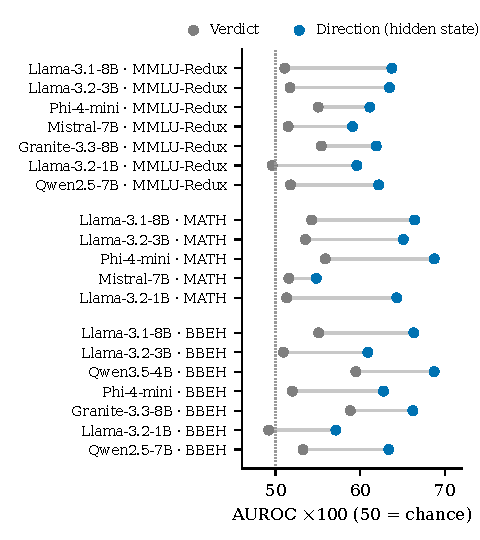
\includegraphics[width=\columnwidth]{fig_gap.pdf}
\caption{Ranking of right above wrong answers to the same question by the judge's verdict and by a linear direction in its hidden state (same answers, out-of-sample direction), for the \R{pool.npairs} judge--benchmark pairs with a gap above 5 points. Not shown (gap $\le 5$): Qwen3.5-9B on all three benchmarks, Qwen3.5-4B on MMLU-Redux and MATH, Granite-3.3-8B and Qwen2.5-7B on MATH, Mistral-7B on BBEH.}
\label{fig:gap}
\end{figure}

The verdicts of small judges rank answers barely above chance: averaged over the \R{pool.npairs} pairs in Figure~\ref{fig:gap}, the verdict's ranking is \R{pool.verdict.rank}. In \R{pool.npairs} of the \R{pairs.all} judge--benchmark pairs the best layer's direction ranks \R{gap.lo} to \R{gap.hi} points higher. The gap is stable: over 20 random splits of the questions its standard deviation is \R{split.sd.lo}--\R{split.sd.hi} points (largest on BBEH, which has about 230 usable questions per half), and the 20-split mean gap is positive for every pair (Appendix Table~\ref{tab:pairs}). The pairs without a gap are mostly the strongest judges: Qwen3.5-9B's verdict already ranks as well as its best direction. The direction peaks in the middle layers (Figure~\ref{fig:layers}, left) and is learned from a few hundred questions with a class-mean difference, so it is not a high-capacity probe that could memorise the answering pool.

\section{Most of It Is Who Wrote the Answer}
\label{sec:author}

Answering models differ in accuracy, so a judge that recognises which model wrote an answer can rank answers well without checking them. We measure how much of a score's variation within a question lies between answering models: the between-model sum of squares divided by the total, within each question, on MMLU-Redux and MATH (BBEH has one answer per model and question). For the direction this share is \R{auth.dir.lo}--\R{auth.dir.hi}\% (median \R{auth.dir.med}\%); for the verdict it is \R{auth.ver.lo}--\R{auth.ver.hi}\%. Both the verdict and the hidden state therefore spend most of their within-question variation telling answering models apart, and much of the gap in Figure~\ref{fig:gap} is the direction separating the more accurate models from the less accurate ones better than the verdict does. In some judges the two disagree in sign: on MMLU-Redux, Llama-3.2-3B accepts only 79\% of Nemotron-3-Super's answers (72\% right) but 98--99\% of Qwen3.5-4B's (43\% right), while its direction ranks Nemotron's answers higher (\S\ref{sec:readout}).

This shortcut is not specific to our setup: any evaluation pool mixing answers from models of different strength rewards it, and self-preference results \citep{panickssery2024llm} show that judges represent authorship. It means that pooled probe accuracies overstate what a judge can check.

\section{Checking Beyond the Judge's Own Ability}
\label{sec:beyond}

\paragraph{Same-model test sets.} For MMLU-Redux and MATH we take the questions Llama-3.1-8B cannot solve and let Qwen3.5-4B answer each 12 more times; we keep questions with at least one right and one wrong answer and up to three of each per question (MMLU-Redux: 2,195 answers to 401 questions; MATH: 1,849 answers to 351 questions). To check that results do not depend on one answering model, OLMo-2-7B-Instruct \citep{olmo2025olmo2}, from a family unrelated to every judge and to Qwen, answers the same questions in the same way. For BBEH, four answering models each contribute up to two right and two wrong of their existing samples per question (2,831 answers to 374 questions). Every compared pair is a right and a wrong answer by the same model to the same question, and each judge is evaluated only on questions it cannot solve itself. The direction is the one learned on the original answer pool (other half of the questions), so nothing is fitted on these sets.

\begin{table*}[t]
\centering
\small
\begin{tabular}{llr r rrrr}
\toprule
& & & & \multicolumn{4}{c}{Gain over the verdict} \\ \cmidrule(l){5-8}
Benchmark & Answers by & Judges & Verdict & Reason & Stretch & Direction & Verdict \\
& & & & first & $\times$11 & & + dir. \\
\midrule
MATH & Qwen3.5-4B & 5 & 57.3 & $-$1.6 & \textbf{+1.7} & \textbf{+2.9} & \textbf{+2.9} \\
MATH & OLMo-2-7B & 5 & 59.9 & $-$2.4 & $-$1.0 & $-$2.3 & $-$0.7 \\
BBEH & Qwen3.5-4B & 6 & 53.6 & $-$0.5 & +0.8 & \textbf{+3.1} & \textbf{+2.1} \\
MMLU-Redux & Qwen3.5-4B & 4 & 46.5 & +1.5 & +0.2 & \textbf{+2.2} & +0.7 \\
MMLU-Redux & OLMo-2-7B & 4 & 50.8 & \textbf{+2.1} & +0.5 & +1.0 & +0.9 \\
\midrule
MATH, failed 9/9$^\dagger$ & Qwen3.5-4B & 1 & 56.8 & $-$0.3 & \textbf{+5.0} & +3.1 & \textbf{+4.7} \\
\bottomrule
\end{tabular}

\caption{Same-model pairs on questions the judge cannot solve: verdict ranking (mean over judges, 50 = chance) and pooled gains of each readout over the verdict. Bold: 95\% interval above 0. $^\dagger$Llama-3.1-8B on the \R{strict.nq} MATH questions it failed in all 9 of its own attempts. Per-judge numbers: Appendix Table~\ref{tab:smpairs}.}
\label{tab:sm}
\end{table*}

\paragraph{Results.} Table~\ref{tab:sm} and Figure~\ref{fig:sm} show three things.

\emph{Verdicts check beyond the judge's ability on reasoning, not on recall.} On MATH questions they cannot solve, the judges rank same-model pairs at \R{sm.math.qwen.verdict.rank} on average for Qwen3.5-4B's answers and \R{sm.math.olmo.verdict.rank} for OLMo-2's, and at \R{sm.bbeh.qwen.verdict.rank} on BBEH. On MMLU-Redux they are at or below chance (\R{sm.mmlu.qwen.verdict.rank} and \R{sm.mmlu.olmo.verdict.rank}). The strongest single case is Llama-3.1-8B on the \R{strict.nq} MATH problems it failed in all nine of its own attempts, where its verdict ranks same-model pairs at \R{strict.verdict.rank}. Checking a worked solution step by step is easier than producing one; recognising a correct multiple-choice letter requires knowing the fact.

\emph{The direction's extra knowledge does not transfer to an unseen answering model.} For Qwen3.5-4B, whose answers are part of the pool the direction is learned from (on other questions), the direction adds to the verdict on all three benchmarks (\R{sm.math.qwen.direct.rank.ci} on MATH, \R{sm.bbeh.qwen.direct.rank.ci} on BBEH, \R{sm.mmlu.qwen.direct.rank.ci} on MMLU-Redux, the last only moving a below-chance ranking toward chance). For OLMo-2, which the direction has never seen, it ranks below the verdict on MATH (\R{sm.math.olmo.direct.rank.ci}) and adds nothing reliable on MMLU-Redux (\R{sm.mmlu.olmo.direct.rank.ci}). Even on same-model pairs, then, part of what the direction encodes is specific to the answering models it was fitted on, consistent with the poor cross-dataset transfer of correctness probes \citep{orgad2025llms,gulati2026auditing}.

\emph{No readout improves checking beyond ability consistently.} Stretching gains on MATH for Qwen's answers (\R{sm.math.qwen.x11.rank.ci}; \R{strict.x11.rank.ci} for Llama-3.1-8B's strict set) but not for OLMo-2's (\R{sm.math.olmo.x11.rank.ci}), and reasoning before the verdict lowers MATH ranking for both answering models (\R{sm.math.qwen.cot.rank.ci} and \R{sm.math.olmo.cot.rank.ci}).

\begin{figure}[t]
\centering
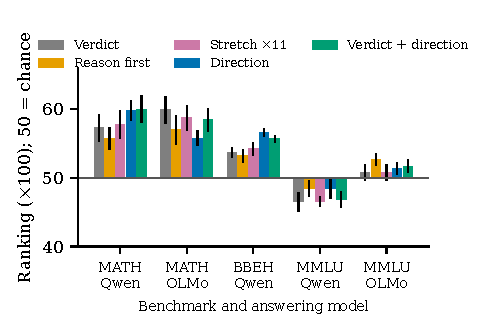
\includegraphics[width=\columnwidth]{fig_sm.pdf}
\caption{Same-model pairs on questions the judge cannot solve: ranking by each readout (mean over judges; bars: standard error over judges).}
\label{fig:sm}
\end{figure}

\section{Getting the Knowledge Out}
\label{sec:readout}

We compare four inference-time readouts with the forced verdict, on the same answers.

\textbf{Reason first.} The judge generates its brief reasoning as the prompt asks (greedy; at most 8,192 tokens on BBEH and 1,536 elsewhere, which \R{cot.reached}\% of runs finish within), and we read the verdict score after its own \texttt{VERDICT:}, appended if it never writes one. \textbf{Direction.} The answer's position along the correctness direction. \textbf{Verdict + direction.} The sum of the verdict score and the direction position, each divided by its within-question standard deviation (no fitted weights). \textbf{Stretch.} We amplify each answer's deviation from the mean along the direction at a single layer, $h \leftarrow h + \beta\,(h^\top v - \mu)\,v$ with $\beta=10$ (``$\times$11''), an activation-steering edit \citep{turner2023steering,li2023iti} that changes the judge's own verdict and output, and read the verdict again.

\paragraph{Choosing the layer for the stretch.} Stretching at the layer where the direction ranks best often fails, because the verdict does not read that layer. A label-free \emph{push test} fixes this: on 400 answers, add $\pm8$ standard deviations of the direction at each layer and measure how far the verdict score moves (its \emph{sensitivity}, in units of the verdict score's within-question spread). Among layers with sensitivity $\ge 0.05$ we stretch the one whose direction ranks best. For Llama-3.1-8B on MATH the best-ranking layer (14) has sensitivity $-0.02$ and stretching there gains $+1.5$; the rule moves to layer 16, where the verdict responds ($+0.26$) and the gain is $+8.2$ (Figure~\ref{fig:layers}). Before running two judges new to the study (Llama-3.2-1B, Qwen2.5-7B) we wrote down this rule and the prediction that every pair with a responding layer gains; it held in 2 of 4 pairs (Appendix~\ref{app:rule}). Overall the stretch gain is significantly positive in \R{pairs.respond.sig} of the \R{pairs.respond} pairs where a layer responds, and a random direction stays within $\pm1$.

\begin{figure*}[t]
\centering
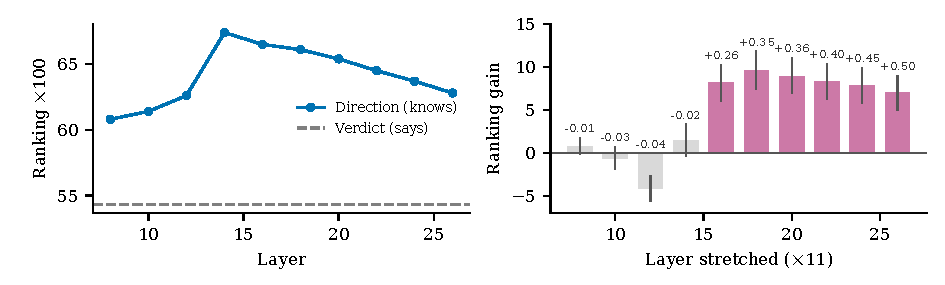
\includegraphics[width=\textwidth]{fig_layers.pdf}
\caption{Llama-3.1-8B on MATH. Left: ranking by the direction learned at each layer, and by the verdict. Right: ranking gain from stretching ($\times$11) at each layer; numbers are the verdict's sensitivity to a push along the direction, and grey bars mark layers below the 0.05 threshold. The best-ranking layer (14) is one the verdict does not read.}
\label{fig:layers}
\end{figure*}

\paragraph{Why the stretch fails when it fails.} Three causes account for the failures among the original judges; the two misses in the fresh test come from choosing among layers whose rankings differ by less than split noise (Appendix~\ref{app:rule}). \emph{Layer too early}: at Llama-3.1-8B's layers $\le 14$ on MATH, pushing the last token moves the accept rate by $\le$2 points, but the same push at every token moves it by up to 16; later layers rebuild the decision from the answer tokens and overwrite a last-token edit. \emph{Verdict reads the direction backwards}: Llama-3.2-3B and Qwen2.5-7B on MMLU-Redux, whose verdicts are negatively correlated with the direction within questions at most layers (the authorship disagreement of \S\ref{sec:author}); no layer responds, and pushing toward ``right'' makes them reject. \emph{Saturated verdict}: Mistral-7B accepts 99\% of MMLU-Redux answers at an average verdict score of $+16.5$, so pushes move the score but never the decision; measuring sensitivity on the score rather than the accept rate fixes this case.

\begin{table*}[t]
\centering
\small
\begin{tabular}{l c rr rr rr rr}
\toprule
& Verdict & \multicolumn{2}{c}{Reason first} & \multicolumn{2}{c}{Stretch $\times$11} & \multicolumn{2}{c}{Direction} & \multicolumn{2}{c}{Verdict + dir.} \\
\cmidrule(lr){3-4}\cmidrule(lr){5-6}\cmidrule(lr){7-8}\cmidrule(l){9-10}
& Rank / BoN & Rank & BoN & Rank & BoN & Rank & BoN & Rank & BoN \\
\midrule
All questions & 53.2 / 61.6 & $-$0.9 & $-$1.4 & \textbf{+2.5} & \textbf{+2.6} & \textbf{+9.2} & \textbf{+8.1} & \textbf{+6.2} & \textbf{+5.5} \\
Judge cannot solve & 50.7 / 58.3 & +0.2 & $-$0.6 & \textbf{+2.4} & \textbf{+2.0} & \textbf{+9.6} & \textbf{+8.9} & \textbf{+6.3} & \textbf{+5.7} \\
\bottomrule
\end{tabular}

\caption{Gains over the forced verdict on the full answer pools (\R{pool.npairs} judge--benchmark pairs, pooled; bold: 95\% interval above 0). Rank: ranking ($\times$100). BoN: best-of-$n$ accuracy, the share of questions (with at least one right and one wrong answer) where the top-scored answer is right; random choice gives \R{pool.random.bon} on all questions.}
\label{tab:readout}
\end{table*}

\paragraph{Comparison.} Table~\ref{tab:readout} compares the readouts on the full answer pools. Reading the direction ranks best (\R{pool.direct.rank.ci} over the verdict) and also picks the right answer more often in best-of-$n$ selection (\R{pool.direct.bon} points); adding it to the verdict comes second, and the stretch recovers only a fraction of the direction's advantage, because only the part of the direction the verdict reads at one layer is amplified. Letting the judge reason before its verdict does not help small judges: it changes ranking by \R{pool.cot.rank.ci} on the full pools and by \R{sm.math.qwen.cot.rank} on same-model MATH pairs. The judges write short justifications (median \R{cot.tok.median} tokens) before committing; the exception is MMLU-Redux, where the forced verdict is at or below chance on same-model pairs and reasoning helps slightly (\R{sm.mmlu.qwen.cot.rank} and \R{sm.mmlu.olmo.cot.rank}). On same-model pairs, ranking gains translate into best-of-$n$ gains only weakly (Appendix~\ref{app:bon}): with three right and three wrong answers from one model, a few points of ranking rarely change which answer is on top.

\section{Does a Larger Judge Close the Gap?}
\label{sec:scale}

\begin{table*}[t]
\centering
\small
\begin{tabular}{l rrr rrr rrr rr}
\toprule
& \multicolumn{3}{c}{MMLU-Redux} & \multicolumn{3}{c}{MATH} & \multicolumn{3}{c}{BBEH} & \multicolumn{2}{c}{Same model} \\
\cmidrule(lr){2-4}\cmidrule(lr){5-7}\cmidrule(lr){8-10}\cmidrule(l){11-12}
Judge & Solves & Verdict & Gap & Solves & Verdict & Gap & Solves & Verdict & Gap & MATH & MMLU \\
\midrule
Llama-3.2-1B & 26 & 49.6 & +12.1 & 3 & 51.9 & +12.8 & 5 & 49.2 & +7.9 & 56.2 & 50.0 \\
Llama-3.2-3B & 35 & 51.7 & +11.6 & 10 & 53.7 & +11.8 & 7 & 50.9 & +10.3 & 62.7 & -- \\
Llama-3.1-8B & 44 & 51.1 & +12.6 & 14 & 54.4 & +13.0 & 10 & 55.1 & +11.2 & 58.3 & 47.5 \\
Llama-3.1-70B & 66 & 65.0 & +1.7 & 30 & 61.9 & +4.4 & 15 & 58.6 & +6.0 & 62.9 & 49.4 \\
\bottomrule
\end{tabular}

\caption{Llama judges by size, on the main answer pools. Solves: share of the pool's questions the judge answers correctly itself (\%). Verdict: the verdict's ranking ($\times$100). Gap: the best layer's direction ranking minus the verdict's. Same model: the verdict's ranking on same-model pairs (Qwen3.5-4B answers) on questions the judge cannot solve; Llama-3.2-3B has no MMLU-Redux same-model run.}
\label{tab:scale}
\end{table*}

We ran Llama-3.1-70B-Instruct through the same pipeline: the same answers, prompts, layer rule and same-model sets (Table~\ref{tab:scale}). Its MMLU-Redux and MATH gaps are below the 5-point threshold, but we ran every step for comparison.

\emph{The verdict improves and the gap shrinks.} The 70B solves \R{scale.70b.mmlu.solved}\% of the MMLU-Redux and \R{scale.70b.math.solved}\% of the MATH questions (Llama-3.1-8B: \R{scale.8b.mmlu.solved}\% and \R{scale.8b.math.solved}\%), and its verdict ranks at \R{scale.70b.mmlu.says}, \R{scale.70b.math.says} and \R{scale.70b.bbeh.says} on the three benchmarks, against \R{scale.8b.mmlu.says}--\R{scale.8b.bbeh.says} for the 8B. Its direction adds only \R{scale.70b.mmlu.gap}, \R{scale.70b.math.gap} and \R{scale.70b.bbeh.gap}, compared with \R{scale.3b.mmlu.gap} to \R{scale.8b.math.gap} for the smaller Llamas on MMLU-Redux and MATH. The larger judge says most of what its hidden state knows. Authorship still accounts for most of both scores' within-question variation (MATH: \R{big.math.auth.dir}\% for the direction, \R{big.math.auth.ver}\% for the verdict).

\emph{Checking beyond the judge's own ability does not grow with size.} On same-model MATH pairs from questions it cannot solve, the 70B's verdict ranks at \R{big.math.sm.qwen.verdict.rank} (Qwen3.5-4B's answers) and \R{big.math.sm.olmo.verdict.rank} (OLMo-2's), within the range of the smaller Llamas (\R{scale.1b.sm.math}--\R{scale.3b.sm.math}). On MMLU-Redux it stays at chance (\R{big.mmlu.sm.qwen.verdict.rank} and \R{big.mmlu.sm.olmo.verdict.rank}), like the 1B (\R{scale.1b.sm.mmlu}). Scale lets a judge check more answers because it knows more answers, not because it gets better at checking the ones it does not know. (Its cannot-solve questions are a harder subset than the small judges', which works against it.)

\emph{The readouts matter less.} On the full pools reading the direction still gains on MATH (\R{big.math.pool.direct.rank.ci}) and BBEH (\R{big.bbeh.pool.direct.rank.ci}). On same-model pairs it neither helps for Qwen's answers (\R{big.math.sm.qwen.direct.rank.ci} on MATH) nor hurts for OLMo-2's (\R{big.math.sm.olmo.direct.rank.ci}); adding it to the verdict gives small gains (\R{big.math.sm.qwen.sum.rank.ci} on MATH, \R{big.bbeh.sm.qwen.sum.rank.ci} on BBEH); stretching does not help and lowers OLMo-2's MATH ranking (\R{big.math.sm.olmo.x11.rank.ci}); reasoning first lowers the pooled MMLU-Redux ranking (\R{big.mmlu.pool.cot.rank.ci}).

\section{Discussion}

\paragraph{What small judges can check.} On reasoning benchmarks, small judges rank same-model answers to problems they cannot solve above chance, for both answering models we tried. This supports the intuition that verification can be easier than generation \citep{cobbe2021training,song2025mind}, and refines the finding that judges agree with experts mainly where they can solve the question \citep{krumdick2026nofreelabels,tan2025judgebench}: the dependence is strong for recall and weaker for worked reasoning. The effect is a few points of AUROC, far smaller than the gaps that pooled evaluations of judges or probes suggest. On recall-heavy questions there is nothing to check without the fact.

\paragraph{Evaluating judges and probes.} A judge, or a probe on a judge, evaluated on answers from models of different strength can score well by recognising authorship, and a probe can keep part of that shortcut even on same-model pairs, as long as the answering model appeared in its training data. Whenever the claim is about checking, we recommend within-question rankings on same-model pairs, on questions the judge cannot solve, from an answering model held out from any fitting.

\paragraph{Using the signal.} On a mixed answer pool, reading the direction or adding it to the verdict is simpler and stronger than amplifying it, and amplifying it at a layer the verdict reads (found by a label-free push test) is the only option that changes the judge's own output. None of these, nor letting the judge reason first, improves checking beyond the judge's own ability consistently across answering models, which is what a weak judge would need most.

\section{Conclusion}

Small LLM judges know more than they say, but most of what they know beyond their verdict is who wrote the answer. Removing authorship and the judge's own ability leaves a smaller, real capacity to check reasoning the judge cannot reproduce, carried by the verdict itself, and none for facts it does not know; the extra knowledge in the hidden state does not survive a change of answering model. A 70B judge says more of what it knows, but is no better at checking what it does not know.

\section*{Limitations}

The main judges have at most 9B parameters and the scale check uses one larger judge (Llama-3.1-70B), whose gap is much smaller, so the readout results matter mainly for small judges; all judges run with thinking disabled, and a reasoning judge may check differently. The same-model sets use questions selected by one judge (Llama-3.1-8B) for MMLU-Redux and MATH, and answers from two answering models; the OLMo-2 MATH set is small (OLMo-2 solves few of these problems: 742 answers to 154 questions). BBEH uses four answering models, all of which also appear in the pool the direction is learned from. Solve labels come from one sample of the judge's own answer, which overstates how often a judge cannot solve a question, except in the strict nine-attempt MATH set. Pooled intervals treat judges as independent although they share questions and answers. The direction needs labelled answers and access to hidden states, which a deployed black-box judge does not offer. Ranking ignores the threshold a deployed judge needs, which stretching shifts. MATH answers are graded by an LLM against reference answers. The layer rule for stretching was revised once after a failure (Mistral-7B) and held in two of four pairs in a fresh test.

\section*{Ethics Statement}

We study open models on public benchmarks and release no new model. Better-calibrated small judges could reduce evaluation costs; the authorship shortcut we document is a risk for any evaluation that relies on LLM judges, and we recommend same-model controls.

\bibliography{refs}

\appendix
\section{Answer Pools}
\label{app:data}

\begin{table}[h]
\centering
\small
\begin{tabular}{llrr}
\toprule
Benchmark & Answering model & Answers & Right \\
\midrule
MMLU-Redux & Qwen3.5-4B & 1,652 & 43\% \\
 & Qwen3.6-35B-A3B & 922 & 81\% \\
 & Nemotron-3-Super-120B & 922 & 72\% \\
\midrule
MATH & Qwen3.5-4B & 1,194 & 50\% \\
 & Qwen3.6-35B-A3B & 602 & 86\% \\
 & Nemotron-3-Super-120B & 588 & 75\% \\
\midrule
BBEH & 8 models & 2,244 & 34--58\% \\
\bottomrule
\end{tabular}
\caption{Main answer pools. BBEH answers come from Qwen3.5-4B, Qwen3.5-9B, Qwen3.6-35B-A3B, Nemotron-3-Nano-30B, Nemotron-3-Super-120B, DeepSeek-V3.1, gpt-oss-20b and gpt-oss-120b. All answers end with a final answer line; MMLU-Redux answers are graded by their final letter against the expert key, MATH answers by GLM-5.3-Flash against the reference (exact matches skip the grader), BBEH answers by the benchmark's matching rule.}
\label{tab:data}
\end{table}

\section{Judge Prompts}
\label{app:prompts}

All judges see one user turn. For MMLU-Redux (MATH and BBEH differ only in the first line: ``a math problem'', ``a reasoning question'', with \texttt{[PROBLEM]} for MATH):

\begin{quote}\small\ttfamily
You are grading an AI assistant's answer to a multiple-choice question.\\[2pt]
[QUESTION]\\ \{question\}\\[2pt]
[ASSISTANT'S ANSWER]\\ \{answer\}\\[2pt]
Is the assistant's final answer correct? Only the final answer matters, not the style of the reasoning. Reason briefly, then end with exactly one line: "VERDICT: CORRECT" or "VERDICT: INCORRECT".
\end{quote}

For the forced verdict and all hidden-state measurements, the assistant turn starts with \texttt{VERDICT:} and we read the next token. For the reasoning baseline, the judge generates freely (greedy, stopping at \texttt{VERDICT:}; at most 8,192 tokens in a 32K window for BBEH and for Llama-3.1-8B on MATH, 1,536 tokens in a 16K window otherwise) and we read the next token after appending \texttt{VERDICT:} to its reasoning. Runs that never write a verdict within the budget (mostly Qwen3.5-4B and Llama-3.1-8B on BBEH, 2--8\% of their answers) are repetitive loops; they are scored the same way. The verdict score uses the first tokens of `` CORRECT'' and `` INCORRECT''.

\section{Layer Rule and Fresh Test}
\label{app:rule}

\paragraph{Rule, fixed before the main run.} Gap check: stop if the gap is $\le 5$. Push test: on 400 random answers, the accept rate at $-8$ and $+8$ standard deviations along the direction at every second layer; a layer responds if the accept rate rises by at least 10 points. Layer: the best-ranking responding layer; if none responds, the best-ranking layer. Stretch: $\times$11 at that layer only, along the direction and along a random direction; $\times$4 and $\times$21 are recorded as secondary readouts.

\paragraph{Revision after a failure.} Mistral-7B on MMLU-Redux accepts 99\% of answers, so no push changes its decision, although the verdict score follows the direction (within-question correlation $+0.54$ to $+0.85$ from layer 18). We therefore measure the response on the verdict score: sensitivity is the mean change in verdict score per standard deviation pushed, divided by the verdict score's within-question standard deviation, and a layer responds if its sensitivity is at least 0.05. This picks the same layer as the original rule wherever the original worked, and layer 16 for Mistral-7B on MMLU-Redux ($+2.3$ [$+0.5$, $+3.7$]).

\paragraph{Fresh test.} Before running Llama-3.2-1B and Qwen2.5-7B, new to the study, we wrote down the revised rule and the prediction that every pair with a gap and a responding layer gains with $\times$11 (interval above 0) and that the random direction stays within $\pm1$. It held for Llama-3.2-1B on MMLU-Redux ($+5.4$) and MATH ($+7.9$), and the random direction stayed within $\pm1$ throughout. It failed on BBEH for both judges ($-1.5$ and $+1.0$). In both, the direction's ranking is flat across the responding layers to within split noise, and the rule took the layer where the verdict only begins to respond; a neighbouring layer with a stronger response gains $+6.4$ [$+3.3$, $+10.3$] (Llama-3.2-1B, layer 14) and $+4.6$ [$+1.2$, $+8.2$] (Qwen2.5-7B, layer 22). Qwen2.5-7B on MMLU-Redux has no responding layer (the backwards-reading failure of \S\ref{sec:readout}).

\paragraph{Strength.} Judges whose verdict responds strongly (sensitivity $\ge 0.2$) do best at $\times$4--$\times$11; weakly responding ones (sensitivity $< 0.08$, mostly BBEH) at $\times$11--$\times$21. $\times$11 is within about two points of the best tested strength for most pairs.

\section{Every Judge and Benchmark}
\label{app:pairs}

\begin{table*}[h]
\centering
\small
\begin{tabular}{ll rr rr rrrr}
\toprule
Bench & Judge & Gap & Gap, 20 splits & Layer & Sens. & Verdict & Reason & Stretch & Direction \\
\midrule
MMLU-Redux & Llama-3.1-8B & +12.6 & +12.2 $\pm$ 0.8 & 16 & 0.13 & 51.1 & 52.6 & 58.0 & 63.7 \\
MMLU-Redux & Llama-3.2-3B & +11.6 & -- & 12$^*$ & 0.06 & 51.7 & 46.5 & 55.8 & 63.4 \\
MMLU-Redux & Qwen3.5-9B & +0.8 & -- & \multicolumn{6}{l}{gap $\le$ 5: not stretched} \\
MMLU-Redux & Qwen3.5-4B & +1.2 & -- & \multicolumn{6}{l}{gap $\le$ 5: not stretched} \\
MMLU-Redux & Phi-4-mini & +7.2 & +7.8 $\pm$ 0.4 & 16 & 0.12 & 55.0 & 52.7 & 58.9 & 61.1 \\
MMLU-Redux & Mistral-7B & +7.6 & +7.9 $\pm$ 0.3 & 4$^*$ & -0.00 & 51.5 & 50.0 & 50.8 & 59.1 \\
MMLU-Redux & Granite-3.3-8B & +6.4 & +5.9 $\pm$ 0.5 & 20 & 0.11 & 55.4 & 51.6 & 57.2 & 61.9 \\
MMLU-Redux & Llama-3.2-1B & +12.1 & +11.7 $\pm$ 0.5 & 10 & 0.05 & 49.6 & 50.9 & 55.0 & 59.6 \\
MMLU-Redux & Qwen2.5-7B & +10.3 & +10.0 $\pm$ 0.7 & 20$^*$ & 0.04 & 51.8 & 50.0 & 54.3 & 62.2 \\
MMLU-Redux & Llama-3.1-70B & +1.7 & +1.4 $\pm$ 0.2 & 34 & 0.27 & 65.0 & 62.6 & 64.9 & 66.8 \\
\midrule
MATH & Llama-3.1-8B & +13.0 & -- & 16 & 0.26 & 54.3 & 53.0 & 62.5 & 66.4 \\
MATH & Llama-3.2-3B & +11.8 & +11.5 $\pm$ 0.4 & 14 & 0.26 & 53.5 & 52.3 & 59.8 & 65.1 \\
MATH & Qwen3.5-9B & +4.9 & -- & \multicolumn{6}{l}{gap $\le$ 5: not stretched} \\
MATH & Qwen3.5-4B & +2.0 & +2.2 $\pm$ 0.3 & \multicolumn{6}{l}{gap $\le$ 5: not stretched} \\
MATH & Phi-4-mini & +12.9 & +12.5 $\pm$ 0.4 & 14 & 0.12 & 55.9 & 56.2 & 62.1 & 68.7 \\
MATH & Mistral-7B & +5.7 & +5.9 $\pm$ 0.7 & 16 & 0.20 & 51.6 & 50.0 & 52.8 & 54.8 \\
MATH & Granite-3.3-8B & +4.4 & +4.5 $\pm$ 0.3 & \multicolumn{6}{l}{gap $\le$ 5: not stretched} \\
MATH & Llama-3.2-1B & +12.8 & +12.1 $\pm$ 1.1 & 14 & 0.15 & 51.3 & 52.5 & 59.1 & 64.3 \\
MATH & Qwen2.5-7B & +5.0 & +5.0 $\pm$ 0.3 & \multicolumn{6}{l}{gap $\le$ 5: not stretched} \\
MATH & Llama-3.1-70B & +4.4 & +4.5 $\pm$ 0.3 & 34 & 0.25 & 61.8 & 62.5 & 62.3 & 66.3 \\
\midrule
BBEH & Llama-3.1-8B & +11.2 & +9.2 $\pm$ 2.3 & 14 & 0.04 & 55.1 & 50.8 & 61.8 & 66.3 \\
BBEH & Llama-3.2-3B & +10.3 & +8.8 $\pm$ 3.1 & 14 & 0.03 & 50.9 & 51.4 & 55.6 & 60.9 \\
BBEH & Qwen3.5-9B & -1.5 & -- & \multicolumn{6}{l}{gap $\le$ 5: not stretched} \\
BBEH & Qwen3.5-4B & +9.3 & +8.0 $\pm$ 1.6 & 20 & 0.08 & 59.5 & 63.9 & 64.7 & 68.7 \\
BBEH & Phi-4-mini & +10.8 & +7.2 $\pm$ 4.2 & 20 & 0.07 & 52.0 & 46.9 & 56.0 & 62.7 \\
BBEH & Mistral-7B & +4.5 & +5.0 $\pm$ 0.8 & \multicolumn{6}{l}{gap $\le$ 5: not stretched} \\
BBEH & Granite-3.3-8B & +7.4 & +6.5 $\pm$ 1.6 & 22 & 0.19 & 58.8 & 53.1 & 65.1 & 66.2 \\
BBEH & Llama-3.2-1B & +7.9 & +5.9 $\pm$ 1.5 & 10 & 0.20 & 49.2 & 52.4 & 47.7 & 57.1 \\
BBEH & Qwen2.5-7B & +10.1 & +8.5 $\pm$ 1.2 & 20 & 0.09 & 53.2 & 54.6 & 54.2 & 63.4 \\
BBEH & Llama-3.1-70B & +6.0 & +4.6 $\pm$ 2.4 & 32 & 0.06 & 58.6 & 57.9 & 60.0 & 64.6 \\
\bottomrule
\end{tabular}

\caption{Every judge--benchmark pair. Gap: best layer's direction ranking minus the verdict's, on the split used for the layer rule; 20 splits: mean $\pm$ standard deviation over 20 random half-splits of the questions (at the best layer). Layer: the layer the rule stretches ($^*$: no layer responds; best-ranking layer). Sens.: the verdict's sensitivity there. Llama-3.1-70B is the scale check of \S\ref{sec:scale}. Last four columns: ranking ($\times$100) of the forced verdict, the verdict after reasoning, the verdict after stretching $\times$11, and the direction, on the main answer pool.}
\label{tab:pairs}
\end{table*}

\begin{table*}[h]
\centering
\small
\begin{tabular}{lll r rrrrrr}
\toprule
Bench & Judge & Answers by & Groups & Verdict & Reason & Str.\,$\times$4 & Str.\,$\times$11 & Direction & Verd.+dir. \\
\midrule
MATH & Llama-3.1-70B & OLMo-2-7B & 89 & 62.6 & 62.8 & 62.6 & 58.9 & 64.4 & 63.3 \\
MATH & Llama-3.1-70B & Qwen3.5-4B & 280 & 62.9 & 63.3 & 63.7 & 63.1 & 64.0 & 64.6 \\
MATH & Llama-3.1-8B & OLMo-2-7B & 154 & 58.9 & 60.5 & 58.6 & 57.9 & 58.9 & 59.0 \\
MATH & Llama-3.1-8B & Qwen3.5-4B & 350 & 58.3 & 57.4 & 62.0 & 62.2 & 60.5 & 61.8 \\
MATH & Llama-3.1-8B & Qwen3.5-4B, failed 9/9 & 255 & 56.8 & 56.5 & 61.6 & 61.8 & 59.9 & 61.6 \\
MATH & Llama-3.2-1B & OLMo-2-7B & 150 & 54.8 & 54.6 & 54.4 & 54.3 & 53.3 & 52.5 \\
MATH & Llama-3.2-1B & Qwen3.5-4B & 340 & 56.2 & 54.4 & 58.3 & 59.9 & 61.8 & 59.9 \\
MATH & Llama-3.2-3B & OLMo-2-7B & 132 & 60.5 & 58.4 & 60.2 & 60.0 & 56.8 & 60.1 \\
MATH & Llama-3.2-3B & Qwen3.5-4B & 327 & 62.7 & 58.8 & 65.3 & 59.4 & 61.3 & 65.3 \\
MATH & Mistral-7B & OLMo-2-7B & 142 & 58.2 & 50.0 & 58.6 & 56.6 & 56.3 & 57.9 \\
MATH & Mistral-7B & Qwen3.5-4B & 262 & 50.7 & 50.0 & 51.2 & 50.6 & 53.9 & 53.3 \\
MATH & Phi-4-mini & OLMo-2-7B & 102 & 67.0 & 61.4 & 66.0 & 64.7 & 53.3 & 62.7 \\
MATH & Phi-4-mini & Qwen3.5-4B & 307 & 58.5 & 57.7 & 60.2 & 56.4 & 61.5 & 59.5 \\
BBEH & Granite-3.3-8B & Qwen3.5-4B & 335 & 50.5 & 51.3 & 53.5 & 53.9 & 56.0 & 54.6 \\
BBEH & Llama-3.1-70B & Qwen3.5-4B & 311 & 55.2 & 58.0 & 56.1 & 54.7 & 56.1 & 57.8 \\
BBEH & Llama-3.1-8B & Qwen3.5-4B & 303 & 54.3 & 50.1 & 54.6 & 55.4 & 55.7 & 56.6 \\
BBEH & Llama-3.2-1B & Qwen3.5-4B & 350 & 53.7 & 53.5 & 54.2 & 49.8 & 55.3 & 54.3 \\
BBEH & Llama-3.2-3B & Qwen3.5-4B & 341 & 53.2 & 54.1 & 55.5 & 54.5 & 55.6 & 54.9 \\
BBEH & Phi-4-mini & Qwen3.5-4B & 343 & 55.7 & 53.8 & 55.9 & 56.6 & 58.7 & 57.3 \\
BBEH & Qwen3.5-4B & Qwen3.5-4B & 210 & 54.4 & 56.2 & 54.8 & 55.2 & 57.9 & 56.2 \\
MMLU-Redux & Granite-3.3-8B & OLMo-2-7B & 193 & 47.7 & 50.4 & 48.8 & 48.7 & 50.6 & 49.1 \\
MMLU-Redux & Granite-3.3-8B & Qwen3.5-4B & 271 & 44.9 & 48.6 & 44.3 & 45.1 & 46.3 & 44.9 \\
MMLU-Redux & Llama-3.1-70B & OLMo-2-7B & 129 & 50.6 & 46.2 & 49.4 & 48.7 & 50.5 & 49.9 \\
MMLU-Redux & Llama-3.1-70B & Qwen3.5-4B & 183 & 49.4 & 50.4 & 49.5 & 46.0 & 48.9 & 49.8 \\
MMLU-Redux & Llama-3.1-8B & OLMo-2-7B & 305 & 53.3 & 52.7 & 53.5 & 53.9 & 53.3 & 53.6 \\
MMLU-Redux & Llama-3.1-8B & Qwen3.5-4B & 401 & 47.5 & 50.3 & 47.8 & 47.5 & 51.0 & 47.4 \\
MMLU-Redux & Llama-3.2-1B & OLMo-2-7B & 241 & 51.5 & 54.6 & 51.1 & 49.5 & 49.3 & 51.9 \\
MMLU-Redux & Llama-3.2-1B & Qwen3.5-4B & 318 & 50.0 & 49.8 & 49.9 & 48.1 & 50.5 & 50.0 \\
MMLU-Redux & Phi-4-mini & OLMo-2-7B & 198 & 50.5 & 53.0 & 50.5 & 50.8 & 51.9 & 52.2 \\
MMLU-Redux & Phi-4-mini & Qwen3.5-4B & 269 & 43.6 & 45.0 & 45.2 & 45.3 & 45.8 & 45.2 \\
\bottomrule
\end{tabular}

\caption{Same-model pairs on questions the judge cannot solve, per judge: ranking ($\times$100) by each readout. Groups: questions with at least one right and one wrong answer from the same answering model.}
\label{tab:smpairs}
\end{table*}

\section{Best-of-$n$ Selection}
\label{app:bon}

\begin{table*}[h]
\centering
\small
\begin{tabular}{lr rr rrrr}
\toprule
Answers & Judges & Random & Verdict & Reason first & Stretch $\times$11 & Direction & Verdict + dir. \\
\midrule
All questions & 19 & 59.8 & 61.6 & $-$1.4 & \textbf{+2.6} & \textbf{+8.1} & \textbf{+5.5} \\
Judge cannot solve & 19 & 58.5 & 58.3 & $-$0.6 & \textbf{+2.0} & \textbf{+8.9} & \textbf{+5.7} \\
Same model, MATH, Qwen3.5-4B & 5 & 56.5 & 63.0 & $-$3.2 & +1.0 & +0.5 & +1.2 \\
Same model, MATH, OLMo-2-7B & 5 & 36.0 & 47.1 & $-$3.6 & $-$1.5 & $-$3.6 & $-$2.8 \\
Same model, BBEH, Qwen3.5-4B & 6 & 47.5 & 50.3 & $-$0.9 & \textbf{+1.5} & \textbf{+2.3} & \textbf{+1.9} \\
Same model, MMLU-Redux, Qwen3.5-4B & 4 & 48.2 & 44.4 & +2.1 & $-$1.2 & +0.2 & $-$1.7 \\
Same model, MMLU-Redux, OLMo-2-7B & 4 & 43.2 & 41.7 & +2.3 & $-$0.5 & +1.4 & +0.7 \\
\bottomrule
\end{tabular}

\caption{Best-of-$n$ accuracy: the share of groups (questions; question $\times$ answering model for same-model sets; only groups with at least one right and one wrong answer) in which the top-scored answer is right, for random choice and the forced verdict, and the gain of each readout over the verdict (pooled over judges; bold: 95\% interval above 0).}
\label{tab:bon}
\end{table*}

\section{Compute}

Hidden-state capture, push tests and stretching ran on single H100 GPUs with Hugging Face Transformers (one forward pass per answer, plus a few edited re-reads of the last token, which can reuse the key-value cache); about one GPU-hour per judge--benchmark pair. Llama-3.1-70B ran on two H200 GPUs on a university cluster (2--3 hours per benchmark for capture, push test and stretching; about 4 hours of vLLM for its own answers and the reasoning baseline). Reasoning judgments and OLMo-2 answers used vLLM. Directions and readouts are computed on CPU from stored hidden states.


\end{document}
